%%%%%%%%%%%%%%%%%%%%%%%%%%%%%%%%%%%%%%%%%%%%%%%%%%%%%%%%%%%%%%%%%%%%%%%%%%%%%%%%
%2345678901234567890123456789012345678901234567890123456789012345678901234567890
%        1         2         3         4         5         6         7         8

%\documentclass{article}
\documentclass[letterpaper, 10 pt, conference]{ieeeconf}  % Comment this line out
                                                          % if you need a4paper
%\documentclass[a4paper, 10pt, conference]{ieeeconf}      % Use this line for a4
                                                          % paper


\overrideIEEEmargins
% See the \addtolength command later in the file to balance the column lengths
% on the last page of the document

\usepackage[utf8x]{inputenc}
\usepackage{cite}
\usepackage{graphicx}
\graphicspath{{figs/}}
\DeclareGraphicsExtensions{.pdf,.jpg,.png}

\usepackage[draft]{fixme}

\title{\LARGE \bf
Explicit Knowledge and the Deliberative Layer: Lessons Learned
}

\author{Séverin Lemaignan and Rachid Alami\\
CNRS-LAAS, 7 av. du Colonel Roche, F-31077 Toulouse, France\\
Université de Toulouse, UPS, INSA, INP, ISAE, LAAS, F-31077 Toulouse, France\\
{\tt surname.name@laas.fr}
}

\begin{document}

\maketitle
\thispagestyle{empty}
\pagestyle{empty}


%%%%%%%%%%%%%%%%%%%%%%%%%%%%%%%%%%%%%%%%%%%%%%%%%%%%%%%%%%%%%%%%%%%%%%%%%%%%%%%%
\begin{abstract}


\end{abstract}


%%%%%%%%%%%%%%%%%%%%%%%%%%%%%%%%%%%%%%%%%%%%%%%%%%%%%%%%%%%%%%%%%%%%%%%%%%%%%%%%
\section{A Knowledge-Oriented Architecture}

\subsection{The LAAS deliberative layer}

\cite{Alami2011}

\begin{figure*}
        \centering
        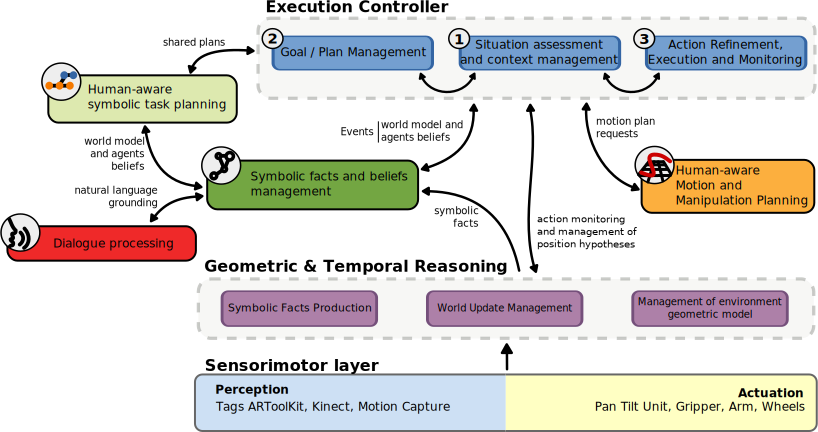
\includegraphics[width=1.7\columnwidth]{archi}
        \caption{Overview of the LAAS deliberative layer.}
        \label{fig|archi}
\end{figure*}

\subsection{Knowledge Model}

\cite{Lemaignan2010}

%%%%%%%%%%%%%%%%%%%%%%%%%%%%%%%%%%%%%%%%%%%%%%%%%%%%%%%%%%%%%%%%%%%%%%%%%%%%%%%%
\section{Situation Assessment}
\label{sect|sit-ass}

\begin{figure}
        \centering
        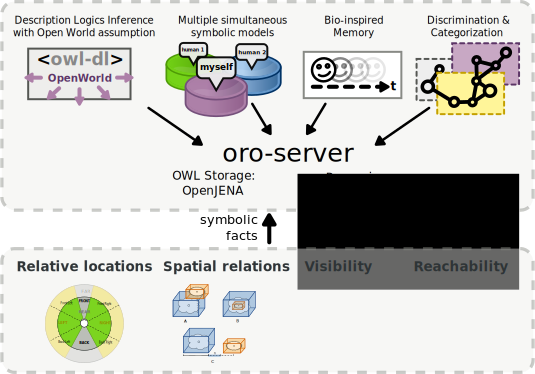
\includegraphics[width=\columnwidth]{spark-oro}
        \caption{Functional overview of knowledge base (\emph{oro-server}, top part) and the geometric situation assessment module (\emph{SPARK}, bottom part)}
        \label{fig|spark-oro}
\end{figure}

\cite{Sisbot2011}

%%%%%%%%%%%%%%%%%%%%%%%%%%%%%%%%%%%%%%%%%%%%%%%%%%%%%%%%%%%%%%%%%%%%%%%%%%%%%%%%
\section{Communication}
\label{sect|com}

\cite{Lemaignan2011a}

\subsection{Disambiguation at semantic level}

\cite{Ros2010b}

\fxnote{Mention failures like 'placeOing'}

\subsection{Multi-modal communication}

%%%%%%%%%%%%%%%%%%%%%%%%%%%%%%%%%%%%%%%%%%%%%%%%%%%%%%%%%%%%%%%%%%%%%%%%%%%%%%%%
\section{Robot Control}
\label{sect|ctrl}

\subsection{Modeling the interaction}

We split the interaction situations stemming from the situation assessment and
communication components in two categories: \emph{desires} and
\emph{experiences}.

\subsection{Task planning}

\cite{Alili2008}

%%%%%%%%%%%%%%%%%%%%%%%%%%%%%%%%%%%%%%%%%%%%%%%%%%%%%%%%%%%%%%%%%%%%%%%%%%%%%%%%
\section{Internal Cognitive Processes}
\label{sect|intern}

\subsection{Theory of Mind}

\cite{Warnier2012a}

\subsection{Working Memory}

%%%%%%%%%%%%%%%%%%%%%%%%%%%%%%%%%%%%%%%%%%%%%%%%%%%%%%%%%%%%%%%%%%%%%%%%%%%%%%%%
\section{Conclusions}
\label{sect|conclusion}

\subsection{The Architect view: loose coupling and modalities merging}

\subsection{The Logician view: the importance of trivial inferences}

\subsection{The Cognician view: palpable knowledge and semantic thinking}

\section*{Acknowledgment}

This work has been supported by EU FP7 ``SAPHARI'' under grant agreement no. ICT-287513.

\bibliographystyle{IEEEtran}
\bibliography{IEEEabrv,biblio}


\end{document}
